\section{Die MAGIC Teleskope}
\label{sec:teleskop}

Die Daten zur Analyse des Krebsnebels werden bereitgestellt durch das MAGIC
(Major Atmospheric Gamma Imaging Cherenkov) Teleskopsystem. Dieses besteht aus
den beiden \SI{17}{\metre} Teleskopen MAGIC I und MAGIC II, die am Roque de
los Muchachos Observatorium auf der Kanareninsel La Palma in einer Höhe von
\SI{2200}{\metre} über dem Meeresspiegel stationiert sind.

\begin{figure}
  \centering
  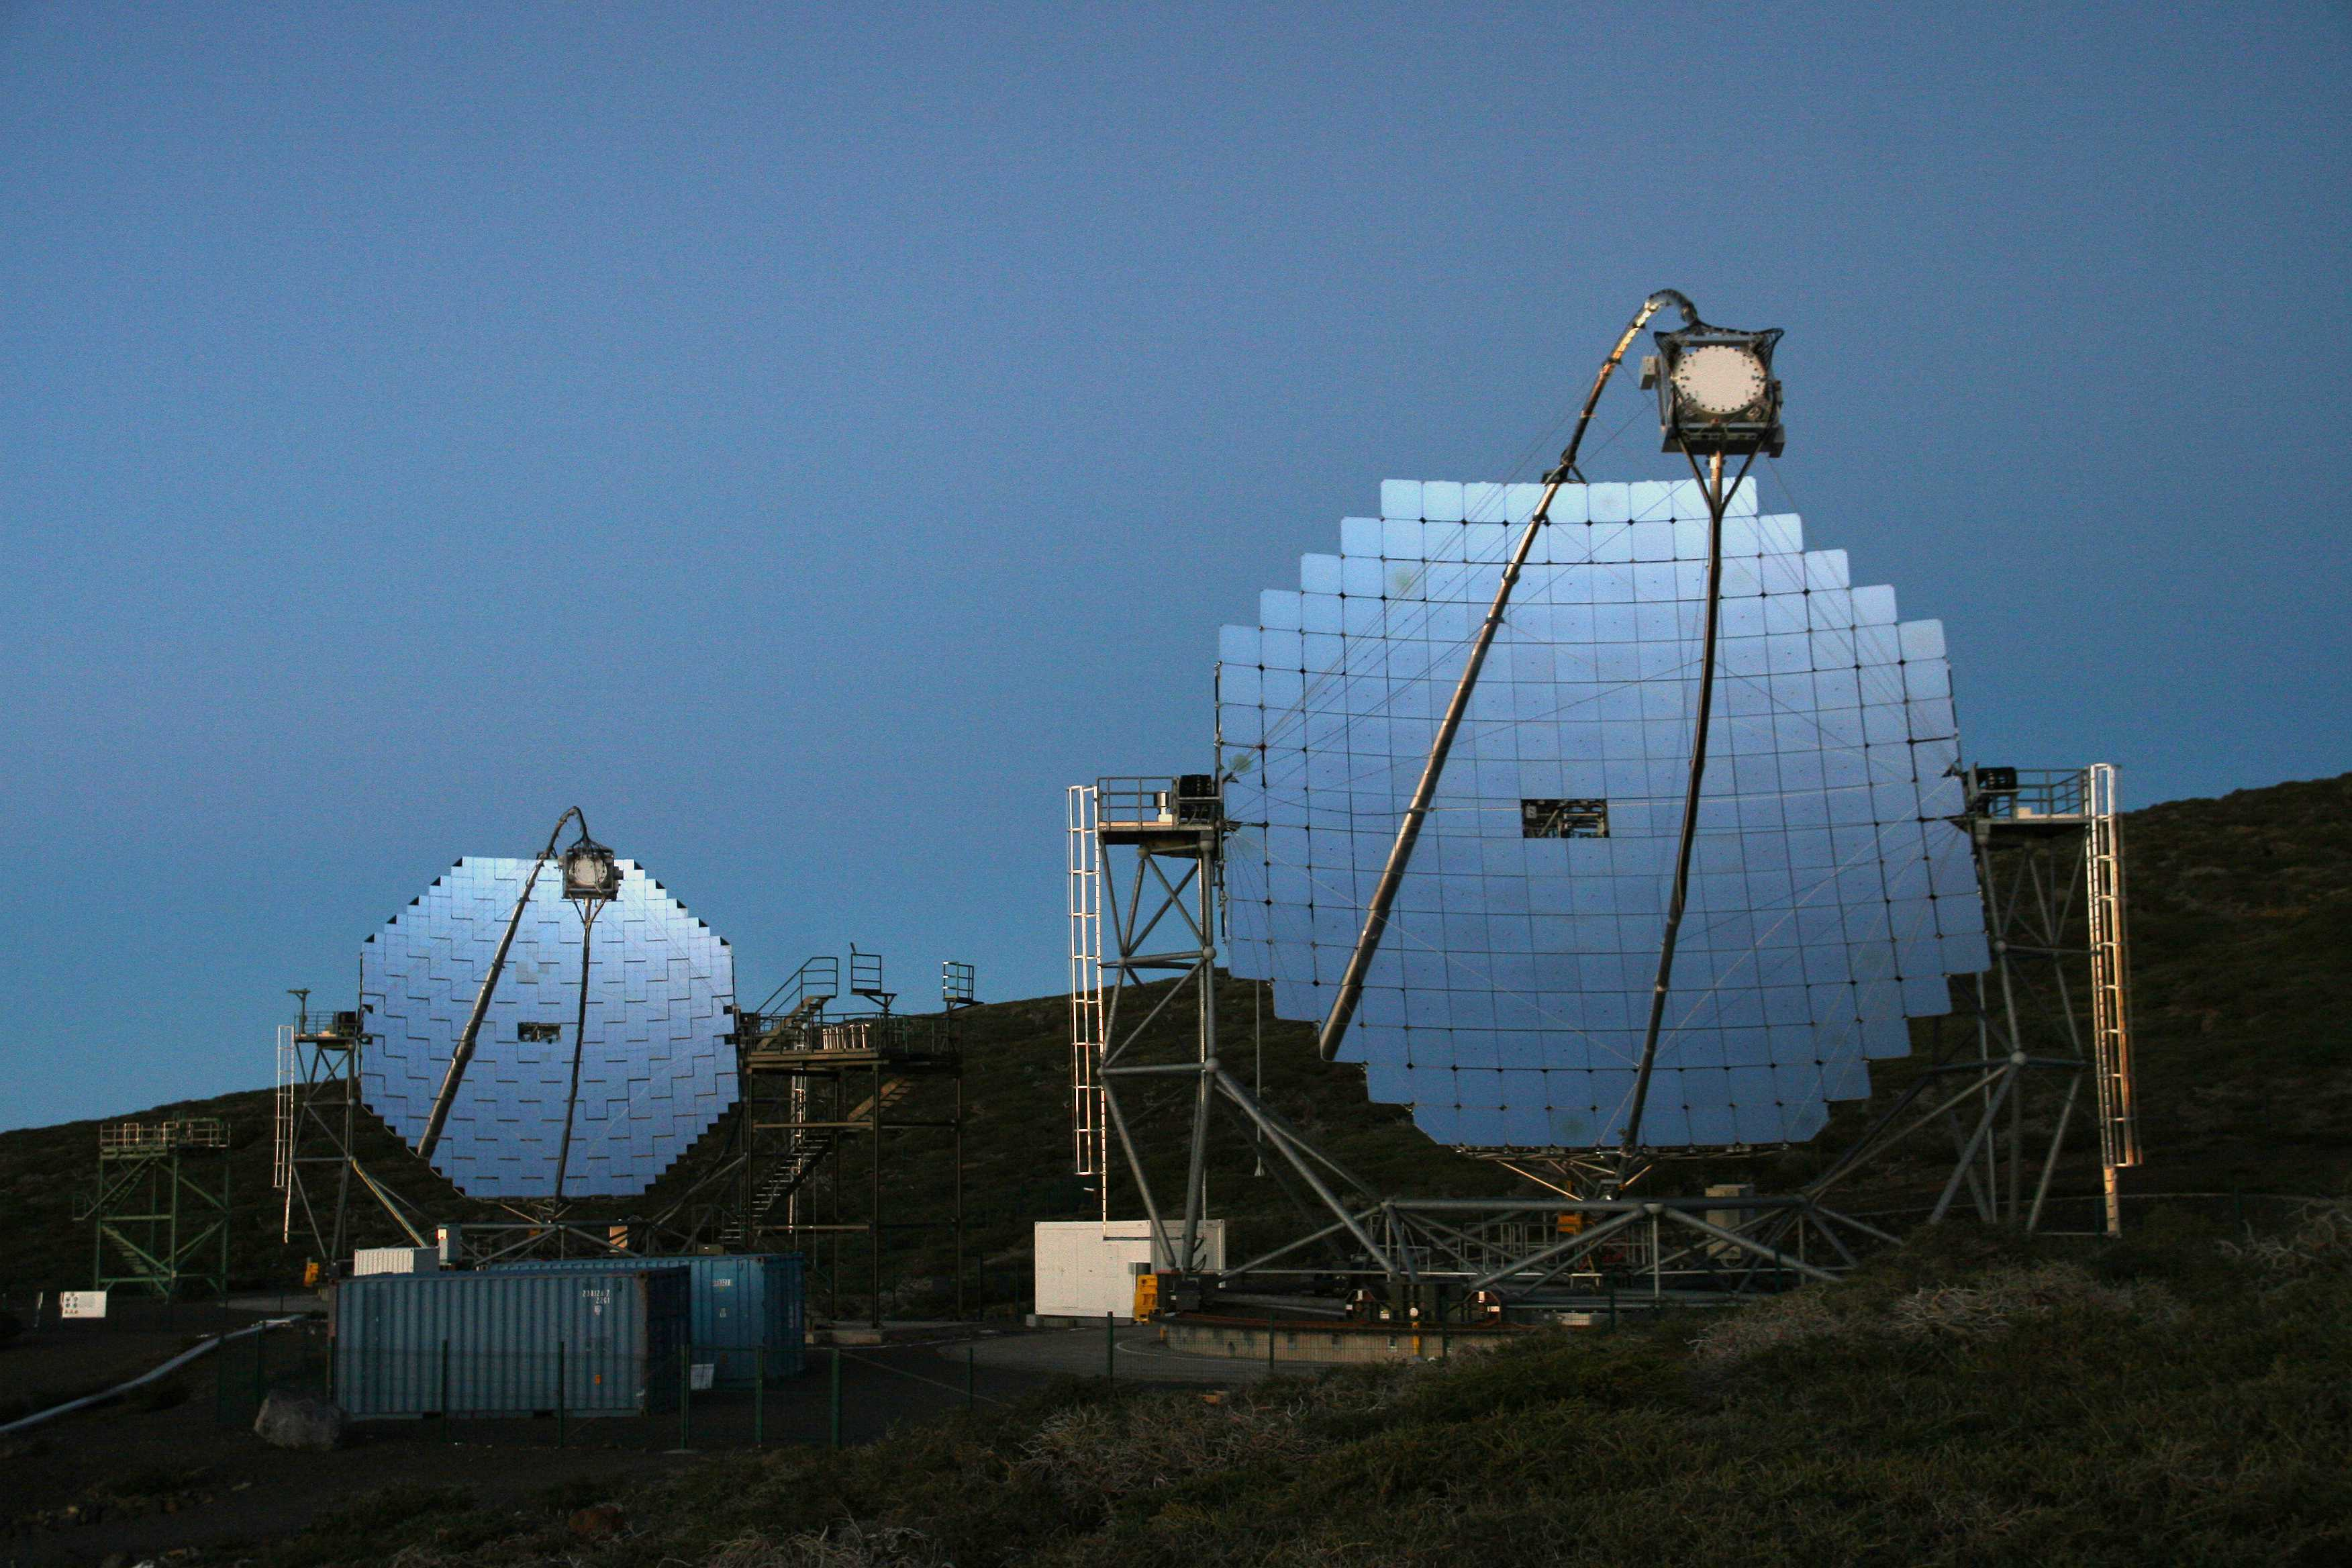
\includegraphics[width=0.65\textwidth]{figures/magic.png}
  \caption{Die zwei MAGIC Teleskope auf der Kanareninsel La Palma. Jedes
  Teleskop hat einen Durchmesser von \SI{17}{\metre}. Im Vordergrund ist
  MAGIC~II zu sehen \cite{magic}.} % Referenz: arxiv:1409.6073v2
  \label{fig:telescope}
\end{figure}

Die MAGIC Teleskope sind spezialisiert auf die Detektion der Tscherenkow-Strahlung
von Teilchenschauern in der Atmosphäre, die durch Gammastrahlung im Energieband
zwischen \SI{50}{\giga\electronvolt} und \SI{50}{\tera\electronvolt} verursacht werden.
Durch die Verwendung von zwei Teleskopen ist eine stereoskopische Beobachtung
möglich, wodurch die Energie und die Einfallsrichtung der primären
Gammastrahlung mit höherer Genauigkeit rekonstruiert werden können. Jedes Teleskop
hat eine aktive Spiegeloberfläche von \SI{239}{\metre\squared}, wobei sich diese
aus quadratischen Einzelspiegeln mit einer Kantenlänge von \SI{50}{\centi\metre}
zusammensetzt. Um Verformungen des Spiegels durch die Elevationsbewegung des
Teleskops zu kompensieren, kann jeder Teilspiegel einzeln justiert werden. Die
kreisförmigen Detektoren bestehen aus je 396 Photomultipliern.

Ziele der MAGIC Kollaboration sind unter anderem die Untersuchung aktiver
galaktischer Kerne (AGN) und die Beobachtung von Supernovaüberresten wie zum
Beispiel des Krebsnebels.
